\begin{figure}[!htb]

    \centering

    \begin{subfigure}[b]{0.49\textwidth}
        \centering
        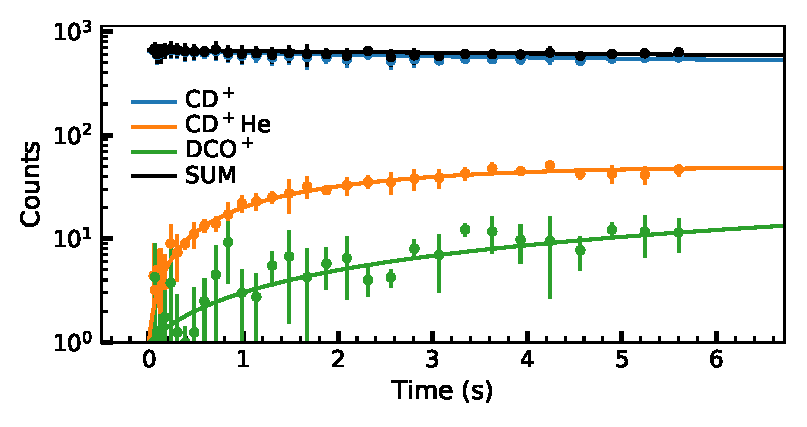
\includegraphics[width=1\textwidth]{figures/measurements/kinetics/loss_channels/m_30_loss_only.pdf}
        \caption{}
        
    \end{subfigure}
    \hfill
    \begin{subfigure}[b]{0.49\textwidth}
        \centering
        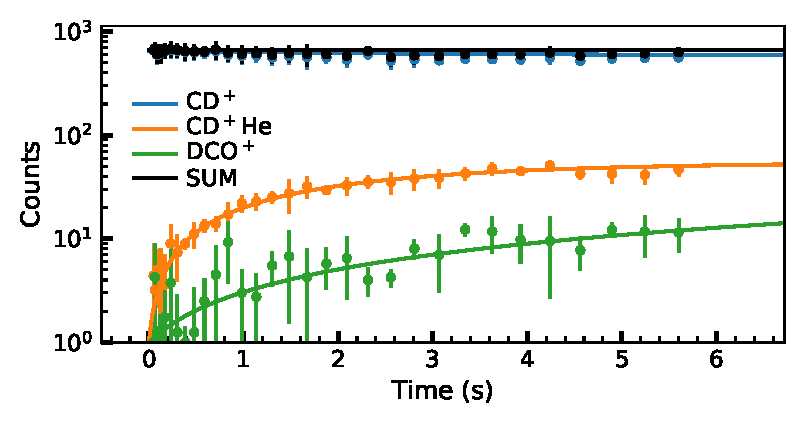
\includegraphics[width=1\textwidth]{figures/measurements/kinetics/loss_channels/trap_and_m_30_loss.pdf}
        % \includegraphics[width=1\textwidth]{figures/measurements/kinetics/compare-loss-channels-additions/without trap loss.pdf}
        \caption{}
        
    \end{subfigure}
    
    \begin{subfigure}[b]{0.49\textwidth}
        \centering
        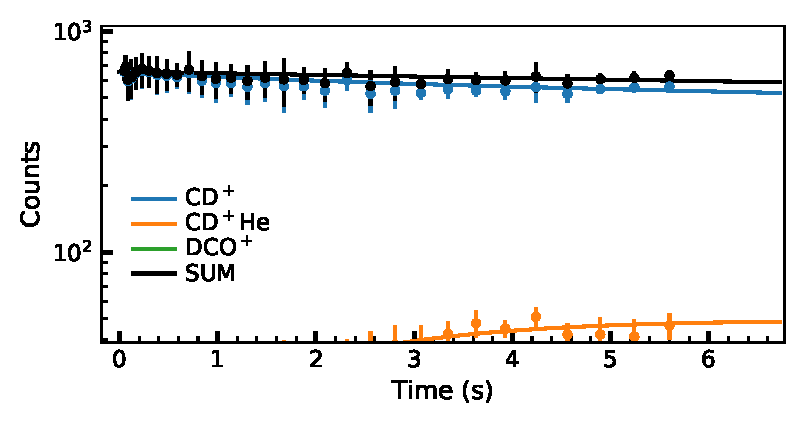
\includegraphics[width=1\textwidth]{figures/measurements/kinetics/loss_channels/m_30_loss_only_zoomed.pdf}
        \caption{}
        
    \end{subfigure}
    \hfill
    \begin{subfigure}[b]{0.49\textwidth}
        \centering
        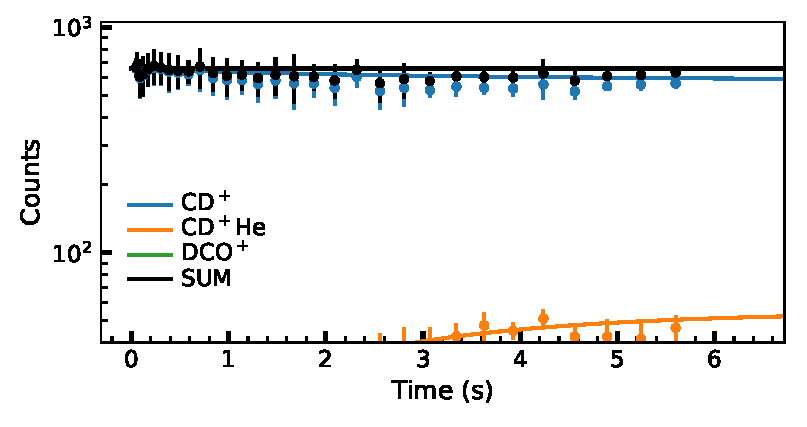
\includegraphics[width=1\textwidth]{figures/measurements/kinetics/loss_channels/trap_and_m_30_loss_zoomed.pdf}
        \caption{}
        
    \end{subfigure}
    
    % \begin{subfigure}[b]{0.49\textwidth}
    %     \centering
    %     \includegraphics[width=1\textwidth]{figures/measurements/kinetics/compare-loss-channels-additions/only mass 30[u] loss.pdf}
    %     \caption{}
    % \end{subfigure}
    
    % \hfill
    % \begin{subfigure}[b]{0.6\textwidth}
    %     \centering
    %     \includegraphics[width=1\textwidth]{figures/measurements/kinetics/compare-loss-channels-additions/trap + mass 30[u] loss.pdf}
    %     \caption{}
        
    % \end{subfigure}
    
    \caption{Comparing loss channels additions: (a) is with both $R_{loss}$ and $R_{loss30}$ channels included while (b) is only with $R_{loss30}$. The (c) and (d) are zoomed-in regions for (a) and (b), respectively. The measurements were carried out at 6.9(3) K and  $1.770(45) \cdot 10^{14}$ \percc\ helium number density. No higher order complexes were formed other than mass 30, which most probably could be DCO$^+$ as described in Eq. \ref{eqn:mass-30-reaction-with-CO2} and \ref{eqn:mass-30-reaction-with-water}}
    
    % \caption{Comparing loss channels additions: (a) is with both $R_{loss}$ and $R_{loss30}$ channels included and no higher order complexes were formed other than mass 30 which most probably could be DCO$^+$ as described in Eq. \ref{eqn:mass-30-reaction-with-CO2} and \ref{eqn:mass-30-reaction-with-water}. The measurement for (a) were carried out at 6.9(3) K and  $1.770(45) \cdot 10^{14}$ \percc helium number density. To compare the effect of including extra trap loss channel, $R_{loss30}$  (b) and (c) are shown, without and with trap loss channel respectively measured at 4.8(3) K and $6.04(25) \cdot 10^{14}$ \percc number density.}
    \label{fig:trap-and-m30-loss-channel-comparision}
\end{figure}